\documentclass[3p,authoryear,11pt,fleqn,review]{elsarticle}
\bibliographystyle{elsarticle-harv}
\usepackage{amsmath,amsfonts,amssymb,siunitx,float,subcaption,setspace,booktabs,diagbox,bm,tikz,mathtools,tikz-3dplot,pgfplots,url}
\usepackage{algorithm}
\usepackage{algpseudocode}
\usepackage{lineno}
\usetikzlibrary{shapes.geometric}
\pgfplotsset{compat=1.8}
\journal{}
\newcommand*{\mb}[1]{\bm{#1}}
\newcommand*{\mT}{\mathrm{T}}
\newcommand*{\md}[1]{\mathrm{d}#1}
\newcommand*{\eqsref}[1]{Eq.~(\ref{#1})}
\newcommand*{\figref}[1]{Fig.~\ref{#1}}
\newcommand*{\tabref}[1]{Table~\ref{#1}}
\newcommand*{\algoref}[1]{Algorithm~\ref{#1}}
\newcommand*{\secref}[1]{\S~\ref{#1}}
\newcommand*{\diag}[1]{\text{diag}\left(#1\right)}
\newcommand*{\sign}[1]{\text{sign}\left(#1\right)}
\newcommand*{\dev}[1]{\text{dev}\left(#1\right)}
\newcommand*{\tr}[1]{\text{trace}\left(#1\right)}
\newcommand*{\ddfrac}[2]{\dfrac{\md{#1}}{\md{#2}}}
\newcommand*{\pdfrac}[2]{\dfrac{\partial{#1}}{\partial{#2}}}
\newcommand{\bsigma}{\mb{\sigma}}
\newcommand{\bvarepsilon}{\mb{\varepsilon}}
\newcommand{\beeta}{\mb{\eta}}
\newcommand{\bn}{\mb{n}}
\newcommand{\balpha}{\mb{\alpha}}
\newcommand{\bbeta}{\mb{\beta}}
\newcommand{\bgamma}{\mb{\gamma}}
\newcommand{\bq}{\mb{q}}
\newcommand{\bs}{\mb{s}}
\newcommand{\bc}{\mb{c}}
\newcommand{\be}{\mb{e}}
\newcommand{\bv}{\mb{v}}
\DeclarePairedDelimiter\abs{\lvert}{\rvert}
\DeclarePairedDelimiter\norm{\lVert}{\rVert}
\makeatletter
\let\oldabs\abs
\def\abs{\@ifstar{\oldabs}{\oldabs*}}
\let\oldnorm\norm
\def\norm{\@ifstar{\oldnorm}{\oldnorm*}}
\newenvironment{breakablealgorithm}
{\begin{center}
\refstepcounter{algorithm}
\hrule height.8pt depth0pt \kern2pt
\renewcommand{\caption}[2][\relax]{
{\raggedright\textbf{\ALG@name~\thealgorithm} ##2\par}
\ifx\relax##1\relax
\addcontentsline{loa}{algorithm}{\protect\numberline{\thealgorithm}##2}
\else
\addcontentsline{loa}{algorithm}{\protect\numberline{\thealgorithm}##1}
\fi
\kern2pt\hrule\kern2pt
}}{\kern2pt\hrule\relax
\end{center}}
\begin{document}
\linenumbers
\begin{abstract}
\begin{linenumbers}
The concept of generalised plasticity theory provides an appealing approach to developing efficient finite element models which could improve computational performance and allow flexibility in customising plastic response.
In this work, we revisit its application in developing frame elements and reformulate a concentrated plasticity frame element to allow its axial force to interact with its end moments ($N$-$M$ interaction).
The proposed element formulation relies on the physical implication of axial plasticity and updates its definition accordingly.
By which, a single axial plasticity history can participate in plasticity evolution and $N$-$M$ interaction at both ends.
The new formulation also redefines the hardening rules to recover desired hardening behaviour, which is not available in the previous formulation.
In terms of numerical performance, the new formulation removes the potential bifurcation issue when both ends experience identical pure axial plasticity history.
The proposed frame element is a high--performing alternative to simulate zero--length plastic hinge frame members that are frequently used in simulations in seismic engineering.
\end{linenumbers}
\end{abstract}
\begin{keyword}
concentrated plasticity frame element\sep
$N$-$M$ interaction\sep
generalised plasticity theory\sep
hysteresis model
\end{keyword}
\begin{frontmatter}
\title{Reformulation of Concentrated Plasticity Frame Element With $N$-$M$ Interaction and Generalised Plasticity}
\author[add1]{Theodore~L.~Chang\corref{tlc}}\ead{tlcfem@gmail.com}
\author[add2]{Chin-Long~Lee}
\cortext[tlc]{corresponding author}
\address[add1]{IRIS Adlershof, Humboldt-Universität zu Berlin, Berlin, Germany, 12489.}
\address[add2]{Department of Civil and Natural Resources Engineering, University of Canterbury, Christchurch, New Zealand, 8041.}
\end{frontmatter}
\section{Introduction}
Beam-column elements are commonly used to simulate the dynamic response of large-scale structures, such as multi-storey buildings and bridges, because of their high computational efficiency compared to continuum finite elements.
By allowing inelastic deformations to distribute within the span, these elements could simulate the spread of inelastic deformations within beams and columns with reasonable accuracy.
This leads to development of distributed inelasticity beam elements, with displacement-based \citep[e.g.,][]{Bathe:96:FEP,Crisfield:97:Book2,Zienkiewicz:Taylor:05:FEM}, force-based \citep[e.g.,][]{Spacone:et:al:96:Fibre,Alemdar2005,Addessi2007,Sideris2016} and mixed formulations \citep[e.g.,][]{Neuenhofer:Filippou:97:Evaluation,Petrangeli:Ciampi:97:Equilibrium,Hjelmstad:Taciroglu:02:Mixed,Taylor:et:al:03:MixedForm,Nukala:White:04:Mixed,DallAsta:Zona:04:Mixed,Lee:Filippou:09:SecInversion}.

In the absence of distributed loads within its body, the element, particularly when used as a column, would likely have its inelastic deformations occur at its ends, where bending moments are the largest.
The efficiency of distributed inelasticity can, therefore, be further optimised by monitoring inelastic deformations only at element ends \citep[e.g.,][]{Attalla:et:al:84:SpreadOP,Scott:Fenves:06:BeamWithHinges,Lee:Filippou:09:SIZE,Scott:Ryan:13:PlasticHinge}.
However, these elements rely on the concept of plastic hinge length, which could be difficult to be parametrised against state variables at element ends, especially for reinforced concrete frames \citep{Park1975,Scott1996}.
This difficulty can be removed by using the concept of concentrated (or lumped) plasticity, where plastic hinges are modelled with zero length.
Such elements are typically called \emph{concentrated plasticity elements}.

The earliest concentrated plasticity elements with this concept include the one-component model \citep{Giberson:67:OneComponent}.
This element was later extended to incorporate the $N$-$M$ interaction (yield surface) via resultant plasticity theory \citep{Orbison:et:al:82:YieldSurface}.
In terms of computing the $N$-$M$ interaction surface, an iterative design procedure was presented by \citet{Liu:et:al:12:CrossSection} for various types of sections.
To incorporate strain hardening, the concept of multiple yield surfaces such as loading and bounding surfaces \citep[e.g.,][]{Iwan:67:Yielding,Mroz:67:AnisoHardening,Mroz:69:GeneralHardening,Dafalias:Popov:75:YieldSurface,Dafalias:Popov:77:YieldSurface} in classic plasticity theory was also adopted \citep[e.g.,][]{Hilmy:Abel:85:PHElement,Hajjar:Gourley:97:PHElement}, usually for modelling steel--concrete composite members.
Among those, the beam model by \citet{Powell:Chen:86:GeneralizedPH} adopts discrete plastic hinges attaching to both end nodes, such that plasticity on two plastic hinges can evolve independently. Thus, each plastic hinge acts as a zero-length connector connecting `internal node' to `external node'.
By borrowing the concept of the generalised plasticity theory \citep{Auricchio1994}, \citet{Kostic:et:al:11:EfficientBCElem0,Kostic:et:al:13:EfficientBCElem,Kostic:et:al:16:GenPlasticity} further extended the formulation by removing the need of internal nodes and proposed a two-node element. Return map algorithms are typically used to ensure element forces stay on the yield surface upon yielding.

Combing the $N$-$M$ interaction and the generalised plasticity theory in the concentrated plasticity elements would cause some challenges given that the $N$-$M$ interaction at each beam end is independent of the other end, but both ends are linked to each other as they share an identical axial force.
In the existing formulation \citep{Kostic:et:al:11:EfficientBCElem0,Kostic:et:al:13:EfficientBCElem,Kostic:et:al:16:GenPlasticity}, due to the adoption of two independent sets of plasticity variables --- one for each node, numerical instability and bifurcation might result when both ends experience the same axial plasticity history. A careful examination reveals that local Jacobian would become singular under certain circumstances.
Due to the coupling between two ends, the hardening rules defined in a conventional manner cannot recover the desired hardening behaviour.
Furthermore, since the hardening parameters do not possess any physical implication, the calibration for their values for a desirable isotropic and kinematic hardening behaviour at either element end is also error--prone.

In this work, we revisit the generalised plasticity framework of the concentrated plasticity beam element and reformulate the $N$-$M$ interactions at each element end such that a desired isotropic and kinematic hardening behaviour can be achieved.
A new definition for axial plastic deformation is also introduced to address the bifurcation issue in the previous formulation.
The reformulation provides a solid theoretical framework that can be extended by adopting more complex plasticity rules to simulate frame members made of various materials.

In the following, the plasticity framework is first introduced with a return mapping type local integration algorithm.
A comparison between the previous \citep{Kostic:et:al:11:EfficientBCElem0} and revised models are then presented with discussions of existing issues and the corresponding improvements.
Numerical examples are investigated to validate and showcase the capability and performance of the proposed formulation.
%
%The conventional plasticity theory is often applied to strain and stress at each integration point. Similar concepts can be applied to other quantities such as cross--sectional/elemental deformation and resultant once the three base stones of plasticity theory, namely, yield function, flow rule and hardening law, are well defined. Based on this idea, \citet{Lubliner1993} proposed the generalised plasticity theory and \citet{Auricchio1994} applied it to membrane/plate problems. Such a framework provides great flexibility in terms of defining nonlinear plastic behaviour of elements and improves numerical performance significantly as there are no integration points involved, the state determination is essentially a single step plasticity integration.
%
%A two--node beam element developed based on the generalised plasticity model is an appealing tool in seismic/structural engineering. It minimises computational cost as there are no sections or material integration points involved. The efficiency of such types of beam elements is significantly higher than traditional displacement/force based fibre type elements. It provides an easy approach to simulate zero-length end plastic hinges. However, combing the $N$-$M$ interaction and the generalised plasticity theory in beam elements introduces new challenges given that the $N$-$M$ interaction at each beam end is relatively independent from the other end, but both ends are linked with each other as they share the \textbf{identical} axial force.
%
%A similar element has been proposed previously \citep{Kostic2013,Kostic2016}. However, its formulation appears to be problematic. In this work, we revisit the generalised plasticity framework and reformulate the previously proposed two--node beam element to enable $N$-$M$ interactions at each beam end and recover the desired both isotropic and kinematic hardening behaviour. By correct the physical implication of axial plastic deformation, a new definition is introduced to remove numerical instability issues the previous formulation has when both ends experience the identical plasticity history.
%
%The plasticity framework is first introduced with a return mapping type local integration algorithm. A comparison between the previous and revised models are then presented with discussions of existing issues and the corresponding improvements. Numerical examples are investigated to validate and showcase the capability and performance of the proposed element.
\section{The $N$-$M$ Frame Element}
\subsection{Preliminaries}
\subsubsection{Definitions and Kinematics}
Consider a two--node beam\footnote{The word `beam' is used interchangeably with `frame' and/or `beam--column'.} element connecting nodes $i$ and $j$ with its rigid body motions removed, the resulting degrees of freedom are axial deformation $u$, rotational deformation $\theta_{z,i}$ of end $i$ and rotational deformation $\theta_{z,j}$ of end $j$, and additional two end rotations, $\theta_{y,i}$ and $\theta_{y,j}$ about the additional normal axis (typically, the weak axis) in case of a 3D beam.
It is assumed that the beam is rigid against torsion (no torsion deformation). An illustration can be seen in \figref{fig:kinematics}.

The elemental deformation vector $\bv$ can then be defined as
\begin{gather}
\bv=\begin{bmatrix}
u&\theta_{z,i}&\theta_{z,j}&\theta_{y,i}&\theta_{y,j}
\end{bmatrix}^\mT
\end{gather}
for 3D beam elements.
Accordingly, the elemental resistance $\mb{q}$ can be defined as
\begin{gather}
\mb{q}=\begin{bmatrix}
P&M_{z,i}&M_{z,j}&M_{y,i}&M_{y,j}
\end{bmatrix}^\mT,
\end{gather}
where $P$ denotes axial force while $M$ denotes end moment.
The corresponding yield forces are denoted as $P^y$, $M_z^y$ and $M_y^y$ and it is assumed, although not a must, both ends have the same yield forces for brevity.
Such definitions of elemental deformation and resistance are independent of the transformation between global and local reference frames, and thus, can be combined with either linear or corotational transformation.
For this reason, the subsequent discussion is confined to the local reference frame only.

The elastic constitutive relationship, denoted by the superscript $\left(\cdot\right)^e$, is conventionally known as
\begin{gather}
\mb{q}=\mb{K}\bv^e,\qquad\text{with}\qquad\mb{K}=\begin{bmatrix}
\dfrac{EA}{L}&\cdot&\cdot&\cdot&\cdot\\[3mm]
\cdot&\dfrac{4EI_z}{L}&\dfrac{2EI_z}{L}&\cdot&\cdot\\[3mm]
\cdot&\dfrac{2EI_z}{L}&\dfrac{4EI_z}{L}&\cdot&\cdot\\[3mm]
\cdot&\cdot&\cdot&\dfrac{4EI_y}{L}&\dfrac{2EI_y}{L}\\[3mm]
\cdot&\cdot&\cdot&\dfrac{2EI_y}{L}&\dfrac{4EI_y}{L}
\end{bmatrix},
\end{gather}
where $L$ is the initial length of beam element, $EA$ is the axial rigidity and $EI$ denotes the flexural rigidity.
\subsubsection{Basic Quantities}
The above definition is widely adopted as the basic quantities of beam elements.
However, it complicates plasticity formulation due to the coupling of (rotational) DoFs. For example, consider the moment $M_{z,i}$ at end $i$, which can be explicitly written as
\begin{gather}\label{eq:redefine}
M_{z,i}=\dfrac{EI_z}{L}\left(4\theta_{z,i}^e+2\theta_{z,j}^e\right),
\end{gather}
the above expression implies that both $\theta_{z,i}$ and $\theta_{z,j}$ contribute to $M_{z,i}$.
Once node $j$ yields, the plasticity developed on far end DoF $\theta_{z,j}$ would also affect near-end moment $M_{z,i}$, thus, it is difficult, if not impossible, to find a yield rotation that corresponds to yield moment $M^y_{z,i}$ by solely using near end rotation $\theta_{z,i}$.

Instead of $\bv$, the proposed formulation is developed based on the following quantity
\begin{gather}\label{nm:kinematics}
\be=\begin{bmatrix}
\varepsilon\\\chi_{z,i}\\\chi_{z,j}\\\chi_{y,i}\\\chi_{y,j}
\end{bmatrix}=\mb{S}\bv,\qquad\mb{S}=\dfrac{1}{L}\begin{bmatrix}
1&\cdot&\cdot&\cdot&\cdot\\
\cdot&4&2&\cdot&\cdot\\
\cdot&2&4&\cdot&\cdot\\
\cdot&\cdot&\cdot&4&2\\
\cdot&\cdot&\cdot&2&4
\end{bmatrix}.
\end{gather}
As a result, the coupling of rotational degrees of freedom is removed. The corresponding stiffness matrix (between $\bq$ and $\be$) becomes a diagonal matrix.
One may observe that the magnitudes of $\chi_i$ and $\chi_j$ correspond to that of sectional curvatures at two ends (using displacement interpolation as in the conventional displacement-based Euler--Bernoulli beam element).
By using this new quantity, it is possible to find a yield curvature $\chi^y$ that corresponds to $M^y$ for each DoF, viz., $M$ is now a univariate function of $\chi$. It is worth noting that the element length $L$ is optionally moved from elasticity matrix $\mb{K}$ to $\be$, hence $\be$ is a strain--like quantity, rather than deformation in the conventional sense.
However, we do not distinguish between those two terminologies and use elemental `deformation' to refer to $\be$ as defined in \eqsref{nm:kinematics}.

For each end, the nodal deformation can be extracted as
\begin{gather}
\be_i=\begin{bmatrix}
\varepsilon\\\chi_{z,i}\\\chi_{y,i}
\end{bmatrix}=\begin{bmatrix}
1&\cdot&\cdot&\cdot&\cdot\\
\cdot&1&\cdot&\cdot&\cdot\\
\cdot&\cdot&\cdot&1&\cdot
\end{bmatrix}\be=\mb{T}_i\be,\qquad
\be_j=\begin{bmatrix}
\varepsilon\\\chi_{z,j}\\\chi_{y,j}
\end{bmatrix}=\begin{bmatrix}
1&\cdot&\cdot&\cdot&\cdot\\
\cdot&\cdot&1&\cdot&\cdot\\
\cdot&\cdot&\cdot&\cdot&1
\end{bmatrix}\be=\mb{T}_j\be,
\end{gather}
or concisely,
\begin{gather}
\be_\aleph=\mb{T}_\aleph\be,
\end{gather}
where subscript $\left(\cdot\right)_\aleph$ denotes either $\left(\cdot\right)_i$ or $\left(\cdot\right)_j$.
In this work, the presence of subscript $\left(\cdot\right)_\aleph$ implies that it is a nodal quantity, the same symbol without subscript $\left(\cdot\right)_\aleph$ denotes its elemental counterpart.
We define $\mb{T}_i$ and $\mb{T}_j$ to be transformation/selection matrices.
The main purpose of adopting $\be$ in the formulation is to decouple nodal response so that plasticity (on rotational DoFs) can be developed \textbf{independently} at each end. By virtue of this one-to-one correspondence, it becomes feasible to acquire a more precise inference regarding the associated plastic deformation. With $\be$, the plasticity characterised by $\chi^p$ developed on one specific DoF does not lead to plastic response on other DoFs, that is, it only affects the response of itself. Furthermore, for that particular DoF, one could assert that the corresponding $M$ has yielded, this is not achievable with $\bv$, as previously discussed.

The nodal elasto-plastic constitutive relationship can now be conveniently expressed as
\begin{gather}
\mb{q}_\aleph=\mb{E}_\aleph\be_\aleph^e=\mb{E}_\aleph\left(\be_\aleph-\be_\aleph^p\right),\qquad\mb{E}_\aleph=\diag{\begin{matrix}
EA&EI_z&EI_y
\end{matrix}}.
\end{gather}
The corresponding elemental version is
\begin{gather}
\mb{q}=\mb{E}\be^e=\mb{E}\left(\be-\be^p\right),\qquad\mb{E}=\diag{\begin{matrix}
EA&EI_z&EI_z&EI_y&EI_y
\end{matrix}}.
\end{gather}

We further rewrite the above expression in the normalised space (normalised by yield force and yield deformation) as
\begin{gather}\label{eq:new_kin}
\mb{\overline{q}}_\aleph=\overline{\be}_\aleph^e=\overline{\be}_\aleph-\overline{\be}_\aleph^p,\qquad\text{or}\qquad
\mb{\overline{q}}=\overline{\be}^e=\overline{\be}-\overline{\be}^p,
\end{gather}
where the overbar $\overline{\left(\cdot\right)}$ denotes the normalised counterpart, for example,
\begin{gather}\label{eq:nm_normalisedq}
\mb{q}_\aleph=\begin{bmatrix}
P^y&\cdot&\cdot\\\cdot&M_z^y&\cdot\\\cdot&\cdot&M_y^y
\end{bmatrix}\mb{\overline{q}}_\aleph.
\end{gather}
The elemental version with subscript $\left(\cdot\right)_\aleph$ omitted in \eqsref{eq:new_kin} holds due to the fact that DoFs are now decoupled.
\subsection{Generalised Plasticity Framework}
The generalised plasticity concept \citep{Auricchio1994} is followed loosely in this work.
However, the two--surface (yield surface and bounding surface) concept is not adopted as the presence of which makes the quantification of hardening behaviour difficult.

The main challenge comes from the fact that $N$-$M$ interaction should be considered at each node, the activation of plasticity (of the moment) at either end should be relatively independent of the other end.
However, as there is only one axial force that is shared between two ends, its plasticity history affects both ends.
Simply adopting a conventional multisurface formulation \citep[see][Chapter 5]{Simo1998} leads to potential local bifurcation issues, as under certain conditions, one surface would become \textbf{redundant}.
In the following, a special formulation that allows independent activation of plasticity at each end while enabling proper hardening behaviour is presented.
\subsubsection{Yield Function}
\paragraph{Nodal Yield Function}
For each end, the nodal resistance $\mb{q}_\aleph$ should be bounded by the corresponding nodal yield surface $f_\aleph$, then, the admissible region is defined by $f_\aleph\leqslant0$ while the inadmissible region is equivalent to $f_\aleph>0$.
For each node, $f_\aleph$ can be simply chosen as
\begin{gather}
f_\aleph=\Phi_\aleph,
\end{gather}
where $\Phi_\aleph=\Phi_\aleph\left(\mb{s}_\aleph,\alpha_\aleph\right)$ is the $N$-$M$ interaction surface based on the shifted resistance $\mb{s}_\aleph=\mb{q}_\aleph-\bbeta_\aleph$ and the equivalent plastic strain $\alpha_\aleph$, $\bbeta_\aleph$ is similar to the concept of back stress in conventional plasticity models, here back resistance that defines the centre of interaction surface.
The $N$-$M$ interaction surface can not only change its location (governed by $\bbeta_\aleph$) but also grow its size (governed by $\alpha_\aleph$) accordingly.
\paragraph{Elemental Yield Function}
The elemental yield surface $f$ should be able to capture the yielding of any ends, a possible option is
\begin{gather}\label{eq:nm_yield}
f=\sum{}\langle{}f_\aleph\rangle=\sum\langle\Phi_\aleph\rangle=\langle\Phi_i\rangle+\langle\Phi_j\rangle,
\end{gather}
The $\langle\cdot\rangle$ symbol denotes the Macaulay bracket.
By \eqsref{eq:nm_yield}, as long as one end yields (or both yield), $f>0$. \eqsref{eq:nm_yield} is closely related to the multisurface plasticity theory \citep[see][Chapter 5]{Simo1998} but not identical.
The exact multisurface plasticity-based formulation \citep{Kostic:et:al:13:EfficientBCElem} would cause local bifurcation as one of $\Phi_\aleph$ becomes redundant under pure axial loading.
By such, a single elemental yield function $f$ can be used to properly capture the yielding of any ends.

Alternatively, a bounding surface concept, which is frequently adopted in models of geomaterials \citep[see, e.g.,][]{Dafalias2004}, concrete and metals, can be used to simulate a more complex evolution of plasticity.
For simplicity, the above single surface formulation is adopted in this work.
It is worth noting that the major discrepancy compared to conventional plasticity models is that plasticity can develop at either end in a \textbf{relatively} independent manner, in the meantime, two ends are linked with each other via the shared axial force.

Often, $f$ is a non-dimensional function of $\bs$ and $\alpha$.
Dimensional analysis shows a plasticity framework based on normalised quantities can simplify both formulation and implementation, thus, in this work, the yield surface $f_\aleph$ is defined as follows instead.
\begin{gather}
f_\aleph=\Phi_\aleph\left(\mb{\overline{s}}_\aleph,\overline{\alpha}_\aleph\right),
\end{gather}
where $\mb{\overline{s}}_\aleph=\mb{\overline{q}}_\aleph-\overline{\bbeta}_\aleph$ with $\mb{\overline{q}}_\aleph$ be the normalised nodal resistance \eqsref{eq:nm_normalisedq} and $\overline{\bbeta}_\aleph$ be the normalised nodal back resistance, viz.,
\begin{gather}
\bbeta_\aleph=\begin{bmatrix}
P^y&\cdot&\cdot\\\cdot&M_z^y&\cdot\\\cdot&\cdot&M_y^y
\end{bmatrix}\overline{\bbeta}_\aleph.
\end{gather}
\subsubsection{$N$-$M$ Interaction Surface}
The \textbf{initial} $N$-$M$ interaction surface is often defined as a non-homogeneous polynomial. For example, for 2D elements, a common option used by \citet{Orbison:et:al:82:YieldSurface} for light- to medium-weight US shapes is
\begin{gather*}
\Phi_\aleph=1.15\left(\overline{P}-\overline{\beta}_P\right)^2+\left(\overline{M}_z-\overline{\beta}_{M_z}\right)^2+3.67\left(\overline{P}-\overline{\beta}_P\right)^2\left(\overline{M}_z-\overline{\beta}_{M_z}\right)^2-c,
\end{gather*}
where $\overline{\beta}_P$ and $\overline{\beta}_{M_z}$ denote the corresponding components of $\overline{\bbeta}_\aleph$, $c$ is a constant (often unity) that determines the initial size of the surface.

Introducing isotropic hardening to the above equation via $c=c\left(\overline{\alpha}\right)$ \citep{Kostic:et:al:11:EfficientBCElem0} indeed introduces hardening into the model but cannot recover the desired hardening behaviour due to the non-homogeneous attribute of $\Phi_\aleph$.
Instead, accounting for the arbitrariness of $\Phi_\aleph$, one can, for example, define the interaction surface to be
\begin{gather}\label{eq:nm_surface_used}
\Phi_\aleph=
1.15\left(\dfrac{\overline{P}-\overline{\beta}_P}{h_P\left(\overline{\alpha}_\aleph\right)}\right)^2+
\left(\dfrac{\overline{M}_z-\overline{\beta}_{M_z}}{h_{M_z}\left(\overline{\alpha}_\aleph\right)}\right)^2+
3.67\left(\dfrac{\overline{P}-\overline{\beta}_P}{h_P\left(\overline{\alpha}_\aleph\right)}\right)^2\left(\dfrac{\overline{M}_z-\overline{\beta}_{M_z}}{h_{M_z}\left(\overline{\alpha}_\aleph\right)}\right)^2-c,
\end{gather}
where $h\left(\overline{\alpha}_\aleph\right)$ is the isotropic hardening function that satisfies the two conditions $h\left(\overline{\alpha}_\aleph\right)\geqslant0$ and $h\left(0\right)=1$.

We further express the interaction surface in its general form as
\begin{gather}\label{eq:nm_interaction}
\Phi_\aleph=\sum_{i=1}^{n}\left(a_i\prod_{r}\left(\dfrac{\overline{r}-\overline{\beta}_r}{h_r\left(\overline{\alpha}_\aleph\right)}\right)^{b_{i,r}}\right)-c,
\end{gather}
where $n$ is the number of terms, $a_i$ is the constant coefficient of each product, $b_{i,r}$ is the order of each bracket and $r$ represents the specific force component $r\in\left(P,~M_z,~M_y\right)$. \eqsref{eq:nm_interaction} serves as the formal definition of the nodal $N$-$M$ interaction surface with hardening.

It is worth noting that $h_P\left(\overline{\alpha}_\aleph\right)$ does not need to be the same as $h_{M_z}\left(\overline{\alpha}_\aleph\right)$.
Different functions can be assigned to different components so that the interaction surface can change its shape during evolution (to mimic anisotropic hardening).
An example is shown in \figref{fig:nm_anisotropic}.
\subsubsection{Flow Rule}
The evolution of plastic deformation $\overline{\be}^p$ shall be linked to the gradient $\mb{g}$ of plastic potential, which is simply taken as $f$, leading to $\mb{g}=\pdfrac{f}{\mb{\overline{q}}}$.
By denoting $\mb{\zeta}=\Gamma\left(\mb{g}\right)$, one can obtain
\begin{gather}\label{eq:nm_flow}
\dot{\overline{\be}^p}=\gamma\mb{\zeta},
\end{gather}
in which $\gamma$ denotes the plastic multiplier.
It must be noted that since $f$ is now based on normalised quantities, $\dot{\overline{\be}^p}$ denotes the normalised plastic deformation increment.
Different options of function $\Gamma\left(\cdot\right)$ are available.
In this work, the simplest form $\mb{\zeta}=\mb{g}=\pdfrac{f}{\mb{\overline{q}}}$, implying the associative flow rule, is chosen, which can be further explicitly expressed as
\begin{gather}\label{eq:nm_flow_a}
\mb{g}=\sum\mb{T}_\aleph^\mT\pdfrac{\langle\Phi_\aleph\rangle}{\mb{\overline{q}}_\aleph}=\mb{T}_i^\mT\pdfrac{\langle\Phi_i\rangle}{\mb{\overline{q}}_i}+\mb{T}_j^\mT\pdfrac{\langle\Phi_j\rangle}{\mb{\overline{q}}_j}.
\end{gather}
It should also be emphasised that only one plastic multiplier $\gamma$ is adopted in the present formulation.
Other options of $\mb{\zeta}$ include
\begin{gather}
\mb{\zeta}=\dfrac{\mb{g}}{\norm{\mb{g}}},
\end{gather}
which has a fixed size (unity) that is beneficial in terms of alleviating potential numerical instability issues when computing the derivative of $\mb{\zeta}$.
\subsubsection{Isotropic Hardening}
For isotropic hardening, $\dot{\overline{\alpha}_\aleph}$ shall be related to some scalar measure of plastic deformation $\dot{\overline{\be}^p}$.
The simplest one would be
\begin{gather}\label{eq:nm_alpha}
\dot{\overline{\alpha}_\aleph}=\norm{\dot{\overline{\be}^p_\aleph}}=\norm{\mb{T}_\aleph\dot{\overline{\be}^p}}=\gamma\norm{\mb{T}_\aleph\mb{\zeta}}.
\end{gather}
The above definition implies that nodal plastic deformation $\dot{\overline{\be}^p_\aleph}$ can be extracted from elemental plastic deformation $\dot{\overline{\be}^p}$ via
\begin{gather}
\dot{\overline{\be}^p_\aleph}=\mb{T}_\aleph\dot{\overline{\be}^p}.
\end{gather}
The elemental equivalent plastic deformation $\dot{\overline{\alpha}}$ is not used in the formulation, and one must be aware of the fact that $\dot{\overline{\alpha}}\neq\dot{\overline{\alpha}}_i+\dot{\overline{\alpha}}_j$ in general cases.
Essentially, $\dot{\overline{\alpha}}_\aleph$ is the length of projection of $\dot{\overline{\be}^p}$ (a 5D vector in deformation space) onto the 3D sub-space.
An illustration of such a projection for 2D elements is depicted in \figref{fig:nm_alpha}.

A popular isotropic hardening rule that adopts a linear hardening base and a saturation \citep{Voce1955} can be defined as
\begin{gather}\label{eq:nm_iso}
h\left(\overline{\alpha}_\aleph\right)=1+H\overline{\alpha}_\aleph+s-se^{-m\overline{\alpha}_\aleph},
\end{gather}
where $H$ is the linear isotropic hardening ratio, $s$ is the saturation level and $m$ controls hardening speed.
In absence of $H$, it is easy to see that
\begin{gather}
\lim\limits_{\overline{\alpha}_\aleph\rightarrow\infty}h\left(\overline{\alpha}_\aleph\right)=1+s.
\end{gather}
Setting either $s=0$ or $m=0$ leads to pure linear isotropic hardening.

In this work, no anisotropic hardening is considered so that
\begin{gather}
h_P\left(\overline{\alpha}_\aleph\right)=h_{M_z}\left(\overline{\alpha}_\aleph\right)=h_{M_y}\left(\overline{\alpha}_\aleph\right)=h\left(\overline{\alpha}_\aleph\right).
\end{gather}
\paragraph{Apparent Hardening Ratio}
Assume the interaction surface incorporates a linear isotropic hardening and is defined as
\begin{gather}
\Phi_\aleph=a\left(\dfrac{\overline{P}-\overline{\beta}_P}{1+H\overline{\alpha}_\aleph}\right)^2-c,
\end{gather}
which is equivalent to
\begin{gather}
\Phi_\aleph=\left(\dfrac{\overline{P}-\overline{\beta}_P}{\sqrt{\dfrac{c}{a}}+\sqrt{\dfrac{c}{a}}H\overline{\alpha}_\aleph}\right)^2-1,
\end{gather}
Noting that $H$ is the hardening ratio defined in plastic deformation--force space, the counterpart, the apparent hardening ratio $\overline{H}$, in deformation--force space is then \citep{Simo1998}
\begin{gather}\label{eq:nm_eqv_iso_hardening}
\overline{H}=\dfrac{\sqrt{\dfrac{c}{a}}H}{1+\sqrt{\dfrac{c}{a}}H}=\dfrac{H}{\sqrt{\dfrac{a}{c}}+H}.
\end{gather}
This is useful in the quantitative verification of the proposed model.
\subsubsection{Kinematic Hardening}
For kinematic hardening, the rate form of back resistance $\overline{\bbeta}$ can be generally expressed as a function of itself and the increment of plastic deformation $\dot{\overline{\be}^p}$,
\begin{gather}
\dot{\overline{\bbeta}}=\Xi\left(\overline{\bbeta},\dot{\overline{\be}^p}\right).
\end{gather}

The bounding type hardening can be achieved by implementing a proper kinematic hardening model explained as follows.
Let the size of back resistance $\overline{\bbeta}$ be bounded by a fixed size denoted by $B_s$, that is
\begin{gather}
\norm{\overline{\bbeta}}\leqslant{}B_s.
\end{gather}
The evolution direction of $\overline{\bbeta}$ is determined by both the current position of $\overline{\bbeta}$ and that of the corresponding projected image (onto the bounding surface), which is revolving around the origin and can be determined by the direction of plastic flow $\dot{\overline{\be}^p}$, meaning that $\dot{\overline{\bbeta}}$ always points to $B_s\dfrac{\dot{\overline{\be}^p}}{\norm{\dot{\overline{\be}^p}}}$.
The evolution speed is governed by how close the current $\overline{\bbeta}$ is to the bounding limit, such a distance is denoted by $D$ and can be characterised by, for example,
\begin{gather}
D=\dfrac{1}{2}-\dfrac{\overline{\bbeta}}{2B_s}\cdot\dfrac{\dot{\overline{\be}^p}}{\norm{\dot{\overline{\be}^p}}},
\end{gather}
which ranges from \num{0} to \num{1}.
The $\cdot$ operator denotes the inner product.

Combing the direction and speed together, accounting for that $\dfrac{\dot{\overline{\be}^p}}{\norm{\dot{\overline{\be}^p}}}=\dfrac{\mb{\zeta}}{\norm{\mb{\zeta}}}$ holds for associative plastic flow, the rate form of $\overline{\bbeta}$ can be expressed as
\begin{gather}\label{eq:nm_bounding_kin}
\dot{\overline{\bbeta}}=\gamma{}D\left(B_s\dfrac{\mb{\zeta}}{\norm{\mb{\zeta}}}-\mb{\overline{\beta}}\right).
\end{gather}
The concept is depicted in \figref{fig:nm_bounding_kin}.
More complex formulations of kinematic hardening of this type are often seen in constitutive models for geomaterials and metals.
\paragraph{Armstrong--Fredrick Type}
By choosing $D=K_a\norm{\mb{\zeta}}$, the above bounding type hardening rule falls back to the Armstrong--Fredrick type \citep{Frederick2007} kinematic hardening that can be expressed as
\begin{gather}\label{eq:nm_kin}
\dot{\overline{\bbeta}}=K_b\dot{\overline{\be}^p}-K_a\norm{\dot{\overline{\be}^p}}\overline{\bbeta}.
\end{gather}
In the above definition, $K_a$ and $K_b=K_aB_s$ are two kinematic hardening ratios.
Setting $K_a=0$ with $K_b\neq0$ leads to pure linear kinematic hardening behaviour.
Alternatively, a Chaboche-type multiplicative model \citep{Chaboche1989} can also be used.
Furthermore, similar to isotropic hardening, different kinematic hardening rules can be assigned to axial/moment components. See the example presented in the appendix.
In this work, \eqsref{eq:nm_kin} is adopted, accounting for both generality and simplicity.
\paragraph{Apparent Hardening Ratio}
Assume a linear kinematic hardening is defined as
\begin{gather}
\dot{\overline{\bbeta}}=K\dot{\overline{\be}^p}.
\end{gather}
The apparent hardening ratio $\overline{K}$ observed in the deformation--force space is then \citep{Simo1998}
\begin{gather}\label{eq:nm_eqv_kin_hardening}
\overline{K}=\dfrac{K}{1+K}.
\end{gather}
This is useful in the quantitative verification of the proposed model.
\subsubsection{Loading/Unloading Conditions}
Since the elemental yield function $f=\sum{}\langle{}f_\aleph\rangle$ defined in this work cannot take negative values, $f\equiv0$ for all admissible states.
The conventional Kuhn--Tucker complementary conditions should be derived based on nodal surfaces accordingly \citep[see][Eq. 5.2.9]{Simo1998}.
In summary,
\begin{enumerate}
\item for all cases, $\gamma\geqslant0$ and $\Phi_i\leqslant0$ and $\Phi_j\leqslant0$,
\item for elastic loading/unloading, $\gamma=0$ and $\Phi_i<0$ and $\Phi_j<0$,
\item for plastic loading, $\gamma>0$ and one of following cases:
\begin{enumerate}
\item node $i$ yields: $\Phi_i=0$ and $\dot{\Phi}_i=0$ and $\Phi_j<0$,
\item node $j$ yields: $\Phi_i<0$ and $\Phi_j=0$ and $\dot{\Phi}_j=0$,
\item both nodes yield: $\Phi_i=0$ and $\dot{\Phi}_i=0$ and $\Phi_j=0$ and $\dot{\Phi}_j=0$,
\end{enumerate}
\item for neutral loading, $\gamma=0$ and one of the same three cases above.
\end{enumerate}
Following the conventional style, the Kuhn--Tucker complementary condition and consistency condition can be expressed as
\begin{gather}
\gamma\Phi_i\Phi_j=0\qquad\text{and}\qquad\gamma\dot{\Phi}_i\dot{\Phi}_j=0.
\end{gather}
\subsubsection{Remarks}
\begin{enumerate}
\item There is only \textbf{one} elemental yield function $f$, which contains \textbf{two} nodal interaction surfaces $\Phi_\aleph$.
\item The flow rule is derived from the unique elemental yield function $f$. Thus, the plastic flow defined in \eqsref{eq:nm_flow} is strictly associative.
This differs from the multisurface plasticity framework.
The resulting plastic deformation $\overline{\be}^p$ is an elemental quantity.
\item The equivalent plastic deformation $\overline{\alpha}_\aleph$ is computed based on part of elemental plastic deformation $\overline{\be}^p$ and may have different histories for two ends.
Furthermore, in general, $\overline{\alpha}\neq\overline{\alpha}_i+\overline{\alpha}_j$.
\item The back resistance $\overline{\bbeta}$ is based on elemental plastic deformation $\overline{\be}^p$.
No matter which end yields, the same evolution rule applies to both elemental and nodal quantities.
\item The conventional fibre-based beam elements have a symmetric tangent stiffness matrix.
Depending on the specific plastic flow and hardening rules used, such symmetry is, in general, not guaranteed for generalised plasticity-based beam elements.
\end{enumerate}
\section{Discrete System}
The discrete local system in vector form is derived in this section for 3D beam elements accounting for five elemental deformation/force components (three nodal components at each end).
In the case of 2D elements, it reduces to three elemental components and two nodal components.
The formulation is almost identical for both 2D and 3D elements. Thus, only the 3D version is presented.
%The conventional return mapping algorithm is adopted.
\subsection{Elastic Loading/Unloading}
By freezing plasticity, one can compute the elemental trial state as
\begin{gather}\label{eq:nm_qa}
\mb{q}^\text{trial}=\mb{q}_n+\mb{E}\left(\be_{n+1}-\be_n\right),
\end{gather}
the nodal normalised version $\mb{\overline{q}}_\aleph^\text{trial}$ can be extracted accordingly via the relationship
\begin{gather}\label{eq:nm_qb}
\mb{T}_\aleph\mb{q}^\text{trial}=\begin{bmatrix}
P^y&\cdot&\cdot\\\cdot&M_z^y&\cdot\\\cdot&\cdot&M_y^y
\end{bmatrix}\mb{\overline{q}}_\aleph^\text{trial}.
\end{gather}

Then trial yield function can be evaluated for each node.
\begin{gather}\label{eq:nm_f_trial}
f_\aleph^\text{trial}=\Phi_\aleph^\text{trial},
\end{gather}
with $\Phi_\aleph^\text{trial}=\Phi\left(\mb{\overline{s}}_\aleph^\text{trial},\overline{\alpha}_{\aleph,n}\right)$ in which $\mb{\overline{s}}_\aleph^\text{trial}=\mb{\overline{q}}_\aleph^\text{trial}-\mb{\overline{\beta}}_{\aleph,n}$.

If $f^\text{trial}=\sum{}\langle{}f_\aleph^\text{trial}\rangle=0$, implying both $\Phi_\aleph^\text{trial}$ are non-positive, indicating both ends are undergoing elastic loading/unloading.
Otherwise, $f^\text{trial}>0$ and local return mapping is required to determine the plastic state to meet conditions $\gamma>0$ and $f=0$.
\subsection{Plasticity Evolution}
For resistance and back resistance, one can obtain the following by using the implicit (backward Euler) integration.
\begin{gather}\label{eq:nm_qc}
\mb{\overline{q}}_{n+1}=\mb{\overline{q}}^\text{trial}-\dot{\overline{\be}^p}=\mb{\overline{q}}^\text{trial}-\gamma\mb{\zeta}_{n+1},\\
\mb{\overline{\beta}}_{n+1}=\mb{\overline{\beta}}_{n}+K_b\gamma\mb{\zeta}_{n+1}-K_a\norm{\gamma\mb{\zeta}_{n+1}}\overline{\bbeta}_{n+1}.
\end{gather}
Along with \eqsref{eq:nm_yield}, \eqsref{eq:nm_flow}, \eqsref{eq:nm_flow_a}, \eqsref{eq:nm_alpha} and \eqsref{eq:nm_iso}, the system is complete.
\subsection{Local Residual}
For 3D beam elements with kinematic hardening, we take
\begin{gather}
\underbrace{\mb{x}}_{13}=\begin{bmatrix}
\underbrace{\mb{\overline{q}}}_{5}&
\underbrace{\mb{\overline{\beta}}}_{5}&
\underbrace{\overline{\alpha}_i}_{1}&
\underbrace{\overline{\alpha}_j}_{1}&
\underbrace{\gamma}_{1}
\end{bmatrix}
\end{gather}
as the local variable with subscript $\left(\cdot\right)_{n+1}$ omitted for brevity, the local residual is
\begin{gather}\label{eq:nm_residual}
\mb{R}=\left\{
\begin{array}{l}
\mb{\overline{q}}-\mb{\overline{q}}^\text{trial}+\gamma\mb{\zeta},\\[1mm]
\left(1+K_a\gamma\norm{\mb{\zeta}}\right)\mb{\overline{\beta}}-\mb{\overline{\beta}}_{n}-K_b\gamma\mb{\zeta},\\[1mm]
\overline{\alpha}_{i}-\overline{\alpha}_{i,n}-\gamma\norm{\mb{T}_i\mb{\zeta}}\\[1mm]
\overline{\alpha}_{j}-\overline{\alpha}_{j,n}-\gamma\norm{\mb{T}_j\mb{\zeta}}\\[1mm]
\langle\Phi_{i}\rangle+\langle\Phi_{j}\rangle,
\end{array}
\right.
\end{gather}
Physically, plasticity evolution can be activated when either end yields or both yield.
Thus, each end shall be considered separately (but not strictly independently due to the shared axial force).
The (plastic) deformation defined in this work can be transformed into the conventional sense via the $\mb{S}$ matrix, see \eqsref{nm:kinematics}.
\subsection{Jacobian}
By treating $\mb{\zeta}$ as an intermediate variable, the Jacobian $\mb{J}$ can be analytically expressed as
\begin{gather}\label{eq:nm_jacobian}
\mb{J}=\pdfrac{\mb{R}}{\mb{x}}+\pdfrac{\mb{R}}{\mb{\zeta}}\ddfrac{\mb{\zeta}}{\mb{g}}\ddfrac{\mb{g}}{\mb{x}},
\end{gather}
where
\begin{gather}
\pdfrac{\mb{R}}{\mb{x}}=\begin{bmatrix}
\mb{I}&\cdot&\cdot&\cdot&\mb{\zeta}\\[2mm]
\cdot&\left(1+K_a\gamma\norm{\mb{\zeta}}\right)\mb{I}&\cdot&\cdot&K_a\norm{\mb{\zeta}}\overline{\bbeta}-K_b\mb{\zeta}\\[2mm]
\cdot&\cdot&1&\cdot&-\norm{\mb{T}_i\mb{\zeta}}\\[2mm]
\cdot&\cdot&\cdot&1&-\norm{\mb{T}_j\mb{\zeta}}\\[2mm]
\mb{\zeta}^\mT&-\mb{\zeta}^\mT&\pdfrac{\langle\Phi_i\rangle}{\overline{\alpha}_i}&\pdfrac{\langle\Phi_j\rangle}{\overline{\alpha}_j}&\cdot
\end{bmatrix},
\end{gather}
and
\begin{gather}
\pdfrac{\mb{R}}{\mb{\zeta}}=\begin{bmatrix}
\gamma\mb{I}\\[4mm]
\dfrac{K_a\gamma}{\norm{\mb{\zeta}}}\overline{\bbeta}\mb{\zeta}^\mT-K_b\gamma\mb{I}\\[4mm]
-\gamma\dfrac{\mb{\zeta}^\mT\mb{T}_i^\mT\mb{T}_i}{\norm{\mb{T}_i\mb{\zeta}}}\\[4mm]
-\gamma\dfrac{\mb{\zeta}^\mT\mb{T}_j^\mT\mb{T}_j}{\norm{\mb{T}_j\mb{\zeta}}}\\[4mm]
\cdot
\end{bmatrix},\qquad
\ddfrac{\mb{g}}{\mb{x}}=\begin{bmatrix}
\pdfrac{\mb{g}}{\mb{\overline{q}}}&-\pdfrac{\mb{g}}{\mb{\overline{q}}}&\pdfrac{\mb{g}}{\overline{\alpha}_i}&\pdfrac{\mb{g}}{\overline{\alpha}_j}&\cdot
\end{bmatrix},
\end{gather}
Note the above expression also takes advantage of the fact that $\pdfrac{}{\mb{\overline{q}}}=-\pdfrac{}{\mb{\overline{\beta}}}$.

The choice of local variable is not unique.
Other options are available.
However, with the above formulation, the Jacobian is greatly simplified at the cost of increasing the size of the local system to \num{13}.
In absence of back resistance $\mb{\overline{\beta}}$, the size reduces to \num{8}.
For 2D beams, those two numbers are \num{9} and \num{6}.
The chosen scheme is believed to be a good balance between analytical expressiveness (simplicity) and numerical performance.
\subsection{Consistent Tangent Operator}
Full differentiation the local residual $\mb{R}$ at equilibrium $\mb{R}=\mb{0}$ gives
\begin{gather}
\pdfrac{\mb{R}}{\be_{n+1}}\md{\be_{n+1}}+\pdfrac{\mb{R}}{\mb{x}}\md{\mb{x}}=\mb{0},
\end{gather}
which leads to the following expression after rearrangement,
\begin{gather}
\ddfrac{\mb{x}}{\be_{n+1}}=-\left(\pdfrac{\mb{R}}{\mb{x}}\right)^{-1}\pdfrac{\mb{R}}{\be_{n+1}},\qquad
\pdfrac{\mb{R}}{\be_{n+1}}=\begin{bmatrix}
-\ddfrac{\mb{\overline{q}}^\text{trial}}{\be_{n+1}}\\\mb{0}\\0\\0\\0
\end{bmatrix},
\end{gather}
with
\begin{gather}
\ddfrac{\mb{\overline{q}}^\text{trial}}{\be_{n+1}}=\diag{\begin{matrix}
P^y&M^y_z&M^y_z&M^y_y&M^y_y
\end{matrix}}^{-1}\mb{E}.
\end{gather}

The consistent tangent operator can then be derived via the chain rule as
\begin{gather}\label{eq:nm_consistent_tangent}
\begin{split}
\ddfrac{\mb{q}_{n+1}}{\be_{n+1}}&=\ddfrac{\mb{q}_{n+1}}{\mb{\overline{q}}_{n+1}}\ddfrac{\mb{\overline{q}}_{n+1}}{\be_{n+1}}=\ddfrac{\mb{q}_{n+1}}{\mb{\overline{q}}_{n+1}}\left(\ddfrac{\mb{x}}{\be_{n+1}}\right)^{\langle1-5\rangle}\\
&=-\diag{\begin{matrix}
P^y&M^y_z&M^y_z&M^y_y&M^y_y
\end{matrix}}\left(\mb{J}^{-1}\pdfrac{\mb{R}}{\be_{n+1}}\right)^{\langle1-5\rangle},
\end{split}
\end{gather}
in which $\left(\cdot\right)^{\langle1-5\rangle}$ denotes the first five rows of target quantity $\left(\cdot\right)$. By further appending a $\mb{S}$ matrix, the consistent tangent operator against $\bv_{n+1}$ can be expressed as
\begin{gather}
\ddfrac{\mb{q}_{n+1}}{\bv_{n+1}}=\ddfrac{\mb{q}_{n+1}}{\be_{n+1}}\ddfrac{\be_{n+1}}{\bv_{n+1}}=\ddfrac{\mb{q}_{n+1}}{\be_{n+1}}\mb{S}.
\end{gather}
\section{Summary of The Proposed Model}
The key expressions of both the previous and proposed models are listed in \tabref{tab:nm_key_eq} for comparison using the notation of this work.
The revisions and the corresponding justifications, along with the resulting improvements, are summarised as follows.
\begin{enumerate}
\item The previous model is developed on dimensional quantities $\bv$ and $\mb{q}$, but the yield surface is non-dimensional, resulting in the associative plastic flow being normalised by yield deformation (dimensionless).
The hardening response then becomes dependent on element rigidities and yield forces.
The new model is formulated in a non-dimensional space ($\overline{\be}$ and $\mb{\overline{q}}$), which corrects the hardening response.
\item The previous model uses \textbf{two} yield functions, each corresponding to an interaction surface.
Each end has its own yield surface and plasticity history. The associative plastic flow is valid for each end but does not hold for elemental quantities since axial plastic deformation needs to be summed up.
The proposed model uses only \text{one} yield function that accounts for both interaction surfaces. The plastic flow is truly associative and is valid at either element or node level.
\item The previous model uses two plastic multipliers ($\gamma_\aleph$) due to two yield surfaces. When two nodes experience identical pure axial plastic history, two yield surfaces give an identical flow direction, making one of the two surfaces redundant. This causes local bifurcation issues.
The proposed model uses one $\gamma$ and is free from local numerical instability.
\item The previous model uses a constant $H$ for isotropic hardening but fails to generate linear isotropic hardening behaviour due to the non-homogeneous attribute of the interaction surface.
The proposed model revises the definition of isotropic hardening and manages to generate the desired isotropic hardening response.
\item The previous model uses inconsistent constitutive expression for $\mb{q}$ and $\bbeta$ as scaling matrix $\mb{\varPi}$ is diagonal while elasticity matrix $\mb{K}$ is not.
The desired kinematic hardening is not achievable.
The proposed model adopts consistent evolution for $\bbeta$.
\item The previous model further adopts a limiting/bounding surface, which was inherited from the generalised plasticity framework in the original literature \citep{Auricchio1994}, to generate a nonlinear hardening response.
The new model achieves a similar response by adopting an Armstrong--Fredrick type kinematic hardening rule instead.
The underlying concept is still a bounding surface but applied to back resistance instead.
\end{enumerate}

An example implementation of the proposed frame element can be seen in \algoref{algo:beam_model}.
Additional stabilisation considerations, such as line search \citep{Dutko1993}, can be accounted for to improve numerical performance.
\begin{breakablealgorithm}
\setstretch{1.2}
\caption{state determination of the proposed frame element}\label{algo:beam_model}
\begin{algorithmic}
\State \textbf{Input}: $\be_{n+1}$, $\be_n$, $\bq_n$, $\overline{\bbeta}_n$, $\overline{\alpha}_{\aleph,n}$
\State \textbf{Output}: $\mb{E}_{n+1}$, $\bq_{n+1}$, $\overline{\bbeta}_{n+1}$, $\overline{\alpha}_{\aleph,n+1}$
\State $\bq^\text{trial}=\bq_n+\mb{E}\left(\be_{n+1}-\be_n\right)$ and transform $\bq^\text{trial}$ to $\overline{\bq}^\text{trial}$
\State $\overline{\bq}_{n+1}=\overline{\bq}^\text{trial}$, $\overline{\bbeta}_{n+1}=\overline{\bbeta}_n$, $\overline{\alpha}_{\aleph,n+1}=\overline{\alpha}_{\aleph,n}$, $\mb{E}_{n+1}=\mb{E}$
\State compute $f$ using $\overline{\bq}_{n+1}$, $\overline{\bbeta}_{n+1}$, $\overline{\alpha}_{\aleph,n+1}$\Comment{\eqsref{eq:nm_f_trial}}
\If {$f>0$}\Comment{plasticity evolution}
\State $\gamma=0$
\While{true}
\State check if each $\Phi_\aleph$ yields or has yielded, assemble $\Phi_\aleph$, $\mb{\zeta}$ and their derivatives
\State compute $\mb{R}$ and $\mb{J}$\Comment{\eqsref{eq:nm_residual} and \eqsref{eq:nm_jacobian}}
\State $\Delta=\left(\mb{J}\right)^{-1}\mb{R}$\Comment{$\Delta=\begin{bmatrix}
\delta\mb{\overline{q}}&
\delta\mb{\overline{\beta}}&
\delta\overline{\alpha}_i&
\delta\overline{\alpha}_j&
\delta\gamma
\end{bmatrix}$}
\If {$\norm{\Delta}<\text{tolerance}$}
\State break
\EndIf
\State $\overline{\bq}_{n+1}\leftarrow\overline{\bq}_{n+1}-\delta\overline{\bq}$
\State $\overline{\bbeta}_{n+1}\leftarrow\overline{\bbeta}_{n+1}-\delta\overline{\bbeta}$
\State $\overline{\alpha}_{\aleph,n+1}\leftarrow\overline{\alpha}_{\aleph,n+1}-\delta\overline{\alpha}_{\aleph}$
\State $\gamma\leftarrow\gamma-\delta\gamma$
\EndWhile
\State transform $\overline{\bq}_{n+1}$ to $\bq_{n+1}$
\State compute $\mb{E}_{n+1}$\Comment{\eqsref{eq:nm_consistent_tangent}}
\EndIf
\end{algorithmic}
\end{breakablealgorithm}

It is worth noting that the particular interaction surface and hardening rules discussed and presented in \tabref{tab:nm_key_eq} are widely recognised and commonly utilised in the modelling of steel. However, when dealing with other materials, it becomes necessary to employ alternative suitable forms.
\section{Numerical Examples}
\subsection{Validation}
As an improved reformulation, in this section, we mainly demonstrate the fact that the proposed formulation is able to produce a desired hardening response.
The cantilever beam has a unit length $L=1$, and all rigidities and yield forces are set to unity, that is, $EA=1$, $EI_z=1$, $P^y=1$ and $M^y_z=1$.
Units are dropped for brevity.
\subsubsection{Isotropic Hardening}
The interaction surface is defined as
\begin{gather}
\Phi=\left(\dfrac{\overline{P}-\overline{\beta}_P}{1+0.1\overline{\alpha}}\right)^2+2\left(\dfrac{\overline{M}_z-\overline{\beta}_{M_z}}{1+0.1\overline{\alpha}}\right)^2-1,
\end{gather}
implying $H=0.1$.
The theoretical hardening ratio can be computed according to \eqsref{eq:nm_eqv_iso_hardening}.
\figref{fig:iso_hardening_a}, \figref{fig:iso_hardening_b} and \figref{fig:iso_hardening_c} present uniaxial cyclic isotropic hardening response under axial force, shear force, and end moment, respectively.
Due to numerical discretisation, some points fall in the transition region(s) and lead to intermediate stiffness values.
They can be ignored.
The desired linear isotropic hardening ratio is properly generated no matter which end yields.
As aforementioned, it is possible to define different hardening functions $h\left(\overline{\alpha}\right)$ for different components to achieve an identical hardening ratio for single DoF loading cases.
However, a unified hardening function ensures the interaction surface grows in size uniformly (isotropic scaling).
\subsubsection{Kinematic Hardening}
The adopted linear kinematic hardening rule is defined as
\begin{gather}
\dot{\overline{\bbeta}}=K\dot{\overline{\be}^p}=0.1\dot{\overline{\be}^p}.
\end{gather}
The theoretical hardening ratio can be computed according to \eqsref{eq:nm_eqv_kin_hardening}.
\figref{fig:kin_hardening_a}, \figref{fig:kin_hardening_b} and \figref{fig:kin_hardening_c} present uniaxial cyclic kinematic hardening response under axial force, shear force, and end moment, respectively.
The target linear kinematic hardening behaviour is also properly generated.
The hardening ratio stays constant (as assigned) for all DoFs, no matter whether one end yields or both ends yield.
\subsection{Calibration}
As mentioned before, in \eqsref{nm:kinematics}, the elemental deformation essentially consists of end-section curvatures and axial strain. It is possible to calibrate the hardening behaviour according to section analysis results in absence of the corresponding experimental data.

An example is presented to show the process by applying moment to a rectangular section.
The section has a geometry of $w\times{}b=12\times1$, the theoretical shape factor of which is \num{1.5}.
This leads to the ultimate moment $M^{ult}=1.5M^y$ assuming material response is purely elastic and perfectly plastic.
By choosing material yield stress $\sigma^y=1$, elastic modulus $E=1$, one can compute $EI_z=2$ and $M^y=2$.

For numerical convenience, \SI{1}{\percent} isotropic hardening is issued to both material models used in section analysis and the proposed beam element.
To reproduce the Bauschinger effect, kinematic hardening is activated with the following parameter: $K_a=1.8$ and $K_b=0.9$.
This gives $B_s=K_b/K_a=0.5$, which meets the shape factor \num{1.5}.

The comparison can be seen in \figref{fig:nm_calibration}.
The overall hysteresis shape can be well captured, and the theoretical maximum moment ($M_{max}=3$) of the section is properly reflected.
Fine--tuning of hardening behaviour can be achieved by, for example, adopting a multiplicative formulation \citep{Chaboche1989}.
The saturation can be associated with the shape factor of the section, which is essentially the ratio between the plastic section modulus and the elastic section modulus, with both usually available in section property tables.
With a specific $N$-$M$ interaction surface, it is possible to adjust the response under various levels of axial loads.
\subsection{A Frame Example}
The performance of the proposed element is compared with that of conventional force-based fibre elements via a response history analysis of a three--storey steel frame structure.
The geometry and dimension of the frame are shown in \figref{fig:nm_frame_hinge}.
The floor mass is \SI{10}{kips\cdot{}s^2/ft} which is lumped on nodes according to tributary length/area and is applied to both horizontal and vertical DoFs.
A uniform damping ratio of \SI{5}{\percent}, which may be high for practical steel structures but is acceptable from the design perspective, using the bell-shaped damping model \citep{Lee2020a,Lee2020b,Lee2021,Lee2022} is defined to cover the response that falls in the frequency range from \SI{0.001}{\radian\per\second} to \SI{1000}{\radian\per\second}, which is sufficient for the target structure with only hardening response.
The material elastic modulus $E$ is set to $E=\SI{29000}{ksi}$ and the yield stress is set to $\sigma^y=\SI{50}{ksi}$.
Those values are used to compute section properties.
Two loads are applied to the structure: 1) vertical gravity load and 2) horizontal earthquake action.
The ground motion used is the normalised accelerogram of the 1940 El Centro earthquake with PGA equal $0.5g$.

The force-based fibre frame element \citep{Spacone1996} is used as the reference element.
The non-iterative algorithm proposed by \citet{Neuenhofer:Filippou:97:Evaluation} is implemented to optimise its computational performance.
Six integration points (sections) along the element chord are used.
For each section, ten integration points along the depth of the section are assigned, resulting in \num{60} material integration points per element.
For the material model, a bilinear hardening model with \SI{1}{\percent} linear isotropic hardening is used.

For the proposed beam element, \SI{1}{\percent} linear isotropic hardening is assigned, and kinematic hardening parameters are determined following the same aforementioned procedure. In specific, the hardening speed $K_a$ is set to unity $K_a=1$, which can be further calibrated, while $K_b/K_a=\dfrac{\text{Plastic Section Modulus}}{\text{Elastic Section Modulus}}-1$.
All section properties are taken from the design manual \citep{AISC2017}. \eqsref{eq:nm_surface_used} is chosen to be the $N$-$M$ interaction surface with $c=1.15$. The comparisons between \eqsref{eq:nm_surface_used} and the ones generated by section analysis is shown in \figref{fig:nm_surface_example}.

The roof drift history is given in \figref{fig:nm_frame_example}.
With the maximum drift being \SI{1.5}{\percent}, significant plasticity is developed as shown in \figref{fig:nm_frame_hinge}, but the drift history shows no significant difference.

In terms of computational cost, for this specific structure, in a parallel context, performing a full response history analysis with the proposed element takes around \SI{30}{\percent} less wall clock time. Note that the number is indicative and may vary depending on different configurations. Excluding the time spent on solving the global matrix, the cost of which is not relevant to element formulations, the proposed element takes around \SI{80}{\percent} less time in terms of sole state determination. Given that the solution of the global matrix typically accounts for a significant portion of the overall computational time, a reduction of \SI{30}{\percent} is regarded as decent.

To close this example, the hysteresis of frame members is presented in \figref{fig:hys}.
It must be pointed out that frame end hysteresis ($\theta_z$-$M_z$) does not reflect whether the target end yields. See the discussion around \eqsref{eq:redefine}.
The responses of components that are not shown (such as the axial forces of middle columns) are purely elastic.

In general, both elements exhibit a comparable hysteresis pattern. As all beams yield, a beam--sway mechanism is formed. However, due to the sensitivity to plastic deformation, the centre of hysteresis may shift by varying amounts.

For a similar bending moment response, the proposed element tends to exhibit larger axial deformation of beams, suggesting that further calibration is necessary for the $N$-$M$ interaction surface. This disparity may arise from multiple sources, including insufficient integration points utilised in fibre elements, inaccurate section discretisation, and varying hardening behaviour attributed to different formulations.

If desired, analysts may perform calibration or implement more sophisticated hardening rules, such as the one presented in the appendix. Nonetheless, as these topics fall beyond the scope of this work, they are not discussed further.

It is worth mentioning that there is no intent to fine-tune the element behaviour to match experimental data on a designation-by-designation basis. Instead, the above structure is presented as a practical example to demonstrate that, without a complex calibration procedure, the proposed element can generate results with a certain level of confidence due to the correct formulation of hardening rules.

Upon comparison with the reference force-based element, it becomes apparent that the results obtained from both elements are similar. There is no plausible reason to indicate that one element is superior to the other. In specific circumstances where the overall response is governed by the strain--stress response at the material level, fibre models tend to necessitate fewer calibration efforts for different members. With the current model, it is required to calibrate $N$-$M$ interaction surfaces on a member-by-member basis.
\section{Conclusions}
In this work, the generalised plasticity theory is revisited and applied to conventional beam elements.
By using a revised yield function, which is able to capture the yielding of either end(s), we formulate an efficient concentrated plasticity beam element that supports the $N$-$M$ interaction, which allows the definition of flexible sectional responses.
The proposed formulation adopts sectional deformations and resultants as the basic quantities and determines the plastic state using a return mapping algorithm.
As evidenced by the frame example, the proposed formulation demonstrates a fairly moderate reduction in computational costs when compared to fibre elements for the presented relatively simple structure.
This renders it an effective and performant tool for simulating lumped plastic hinges at beam ends with zero hinge length.

By properly accounting for the special constraint that the axial force is unique but shared between two end nodes, the hardening behaviour is corrected.
The proposed element shows desired isotropic/kinematic hardening response.
The hardening parameters are now tightly associated with physical implications, making the calibration more reliable.
As the presented hardening laws are suitable for steel beams/columns, practical examples are presented to showcase that the proposed element can be used in response history analysis of steel frames without a complex calibration procedure of model parameters.
It is imperative to note that the exact plastic rules delineated in this study are exclusively applicable to a particular case of steel members with a bilinear material stress--strain law, and are not suitable for sections made of alternative materials, such as reinforced concrete.
Nevertheless, with the proposed formulation, other plastic rules and interaction surfaces can be adopted to simulate other types of frames.
The formulation itself does not impose any restrictions in this regard.
It provides an alternative to conventional beam elements with flexibility for response history analysis.

As sectional quantities are employed as the basic quantities, the corresponding calibration of model parameters (hardening rules and $N$-$M$ interactions) should be carried out based on the corresponding experimental data of member tests or accurate sectional analysis results (in absence of experimental data), if the proposed model is to be used in predictive simulations.

The proposed beam elements (both 2D and 3D versions) are implemented in \texttt{suanPan} \citep{Chang2022}, and all numerical examples are analysed using the same application.
\appendix
\section{Component Based Kinematic Hardening Rule}
Consider a 3D frame element with singly symmetric section geometry, as in general the shape factor, which corresponds to the saturation level defined in the kinematic hardening rule, would have different values along different axes, it is desired to assign different hardening rules for different components.

A simple modification of \eqsref{eq:nm_kin} can be expressed as
\begin{gather}
\dot{\overline{\bbeta}}=\begin{bmatrix}
K_{b,P}&\cdot&\cdot\\
\cdot&K_{b,M_z}&\cdot\\
\cdot&\cdot&K_{b,M_y}
\end{bmatrix}\dot{\overline{\be}^p}-\begin{bmatrix}
K_{a,P}&\cdot&\cdot\\
\cdot&K_{a,M_z}&\cdot\\
\cdot&\cdot&K_{a,M_y}
\end{bmatrix}\norm{\dot{\overline{\be}^p}}\overline{\bbeta}.
\end{gather}
The $K_a$ and $K_b$ pairs can be independently calibrated for each component to match the corresponding section properties of strong/weak axes.

Furthermore, consider an idealised bilinear material model, under pure axial deformation, the axial force resistance follows the material model and generates a bilinear response. However, under pure bending deformation, the end moment develops plasticity gradually and generates a non-linear response, which asymptotically approaches the plastic moment after yielding. One can set $K_{a,P}=0$, $K_{a,M_z}\neq0$ and $K_{a,M_y}\neq0$ so that axial back resistance evolves linearly while bending resistance evolves non-linearly. A graphical illustration of 2D elements is given in \figref{fig:nm_component_kin}.
\section*{Data Availability Statement}
Some or all data, models, or code that support the findings of this study are available from the corresponding author upon reasonable request.
The corresponding model scripts are available online\footnote{\url{https://github.com/TLCFEM/nm-formulation}}.
\bibliography{BIB}
\clearpage
\begin{table}[H]
\centering\footnotesize\renewcommand{\arraystretch}{2}
\caption{Summary of key expressions and parameters.}\label{tab:nm_key_eq}
\begin{tabular}{r|l|l}
    \toprule
                        & previous model \citep{Kostic:et:al:13:EfficientBCElem}                                  & revised model                                                                                                                                                   \\ \midrule
       nodal extraction &                                                                                         & $\left(\cdot\right)_\aleph=\mb{T}_\aleph\left(\cdot\right)$ for all nodal quantities                                                                            \\
             kinematics & $\mb{q}=\mb{K}\left(\bv-\bv^p\right)$                                                   & $\mb{\overline{q}}=\overline{\be}-\overline{\be}^p$                                                                                                             \\
          yield surface & $f_\aleph=\Phi_\aleph-H\alpha_\aleph$                                                   & $f=\langle\Phi_i\rangle+\langle\Phi_j\rangle$                                                                                                                   \\
    interaction surface & $\Phi_\aleph=\Phi_\aleph\left(\mb{q}_\aleph,\bbeta_\aleph\right)$                       & $\Phi_\aleph=\Phi_\aleph\left(\mb{\overline{q}}_\aleph,\mb{\overline{\beta}}_\aleph,\overline{\alpha}_\aleph\right)$                                            \\
                        & $\Phi_\aleph=\sum_{i=1}^{n}\left(a_i\prod_{r}\left(r-\beta_r\right)^{b_{i,r}}\right)-c$ & $\Phi_\aleph=\sum_{i=1}^{n}\left(a_i\prod_{r}\left(\dfrac{\overline{r}-\overline{\beta}_r}{h_r\left(\overline{\alpha}_\aleph\right)}\right)^{b_{i,r}}\right)-c$ \\
              flow rule & $\dot{\overline{\bv}^p_\aleph}=\gamma_\aleph\pdfrac{f_\aleph}{\mb{q}_\aleph}$           & $\dot{\overline{\be}^p}=\gamma\mb{\zeta}=\gamma\pdfrac{f}{\mb{\overline{q}}}$                                                                                   \\
    isotropic hardening & $\dot{\overline{\alpha}_\aleph}=\norm{\dot{\overline{\bv}^p_\aleph}}$                   & $\dot{\overline{\alpha}_\aleph}=\norm{\dot{\overline{\be}^p_\aleph}}=\norm{\mb{T}_\aleph\dot{\overline{\be}^p}}=\gamma\norm{\mb{T}_\aleph\mb{\zeta}}$           \\
                        &                                                                                         & $h\left(\overline{\alpha}_\aleph\right)=1+H\overline{\alpha}+s-se^{-m\overline{\alpha}_\aleph}$                                                                 \\
    kinematic hardening & $\dot{\overline{\bbeta}_\aleph}=K\mb{\varPi}\dot{\overline{\bv}^p_\aleph}$              & $\dot{\overline{\bbeta}}=K_b\dot{\overline{\be}^p}-K_a\norm{\dot{\overline{\be}^p}}\overline{\bbeta}$                                                           \\ \bottomrule
\end{tabular}
\end{table}
\clearpage
\begin{Large}
Please note 15 figures are in the main body. Only the second last one is in the appendix. Please make proper adjustments if needed.
\end{Large}
\listoffigures
\begin{figure}[p]
\centering
\includegraphics[page=1]{PICCOLLECTION}
\caption{Deformation and resistance of a 2D beam.}\label{fig:kinematics}
\end{figure}
\begin{figure}[p]
\centering\footnotesize
\includegraphics[page=2]{PICCOLLECTION}
\caption{Mixed evolution of an example $N$-$M$ interaction surface.}\label{fig:nm_anisotropic}
\end{figure}
\begin{figure}[p]
\centering\footnotesize
\includegraphics[page=3]{PICCOLLECTION}
\caption{Definition of nodal equivalent plastic deformation of 2D beam.}\label{fig:nm_alpha}
\end{figure}
\begin{figure}[p]
\centering\footnotesize
\includegraphics[page=4]{PICCOLLECTION}
\caption{Bounded evolution of nodal back resistance of a 2D beam.}\label{fig:nm_bounding_kin}
\end{figure}
\begin{figure}[p]
\centering\footnotesize
\includegraphics[page=5]{PICCOLLECTION}
\caption{Isotropic hardening validation for axial force.}\label{fig:iso_hardening_a}
\end{figure}
\begin{figure}[p]
\centering\footnotesize
\includegraphics[page=6]{PICCOLLECTION}
\caption{Isotropic hardening validation for transverse force.}\label{fig:iso_hardening_b}
\end{figure}
\begin{figure}[p]
\centering\footnotesize
\includegraphics[page=7]{PICCOLLECTION}
\caption{Isotropic hardening validation for moment.}\label{fig:iso_hardening_c}
\end{figure}
\begin{figure}[p]
\centering\footnotesize
\includegraphics[page=8]{PICCOLLECTION}
\caption{Kinematic hardening validation for axial force.}\label{fig:kin_hardening_a}
\end{figure}
\begin{figure}[p]
\centering\footnotesize
\includegraphics[page=9]{PICCOLLECTION}
\caption{Kinematic hardening validation for transverse force.}\label{fig:kin_hardening_b}
\end{figure}
\begin{figure}[p]
\centering\footnotesize
\includegraphics[page=10]{PICCOLLECTION}
\caption{Kinematic hardening validation for moment.}\label{fig:kin_hardening_c}
\end{figure}
\begin{figure}[p]
\centering\footnotesize
\includegraphics[page=11]{PICCOLLECTION}
\caption{Calibration of hardening according to section analysis result.}\label{fig:nm_calibration}
\end{figure}
\begin{figure}[p]
\centering\footnotesize
\includegraphics[page=12]{PICCOLLECTION}
\caption{Frame setup and plastic hinge distribution.}\label{fig:nm_frame_hinge}
\end{figure}
\begin{figure}[p]
\centering\footnotesize
\includegraphics[page=13]{PICCOLLECTION}
\caption{Comparisons of initial NM interaction curves.}\label{fig:nm_surface_example}
\end{figure}
\begin{figure}[p]
\centering\footnotesize
\includegraphics[page=14]{PICCOLLECTION}
\caption{Roof drift history using fibre element and the proposed element.}\label{fig:nm_frame_example}
\end{figure}
\begin{figure}[p]
\centering\footnotesize
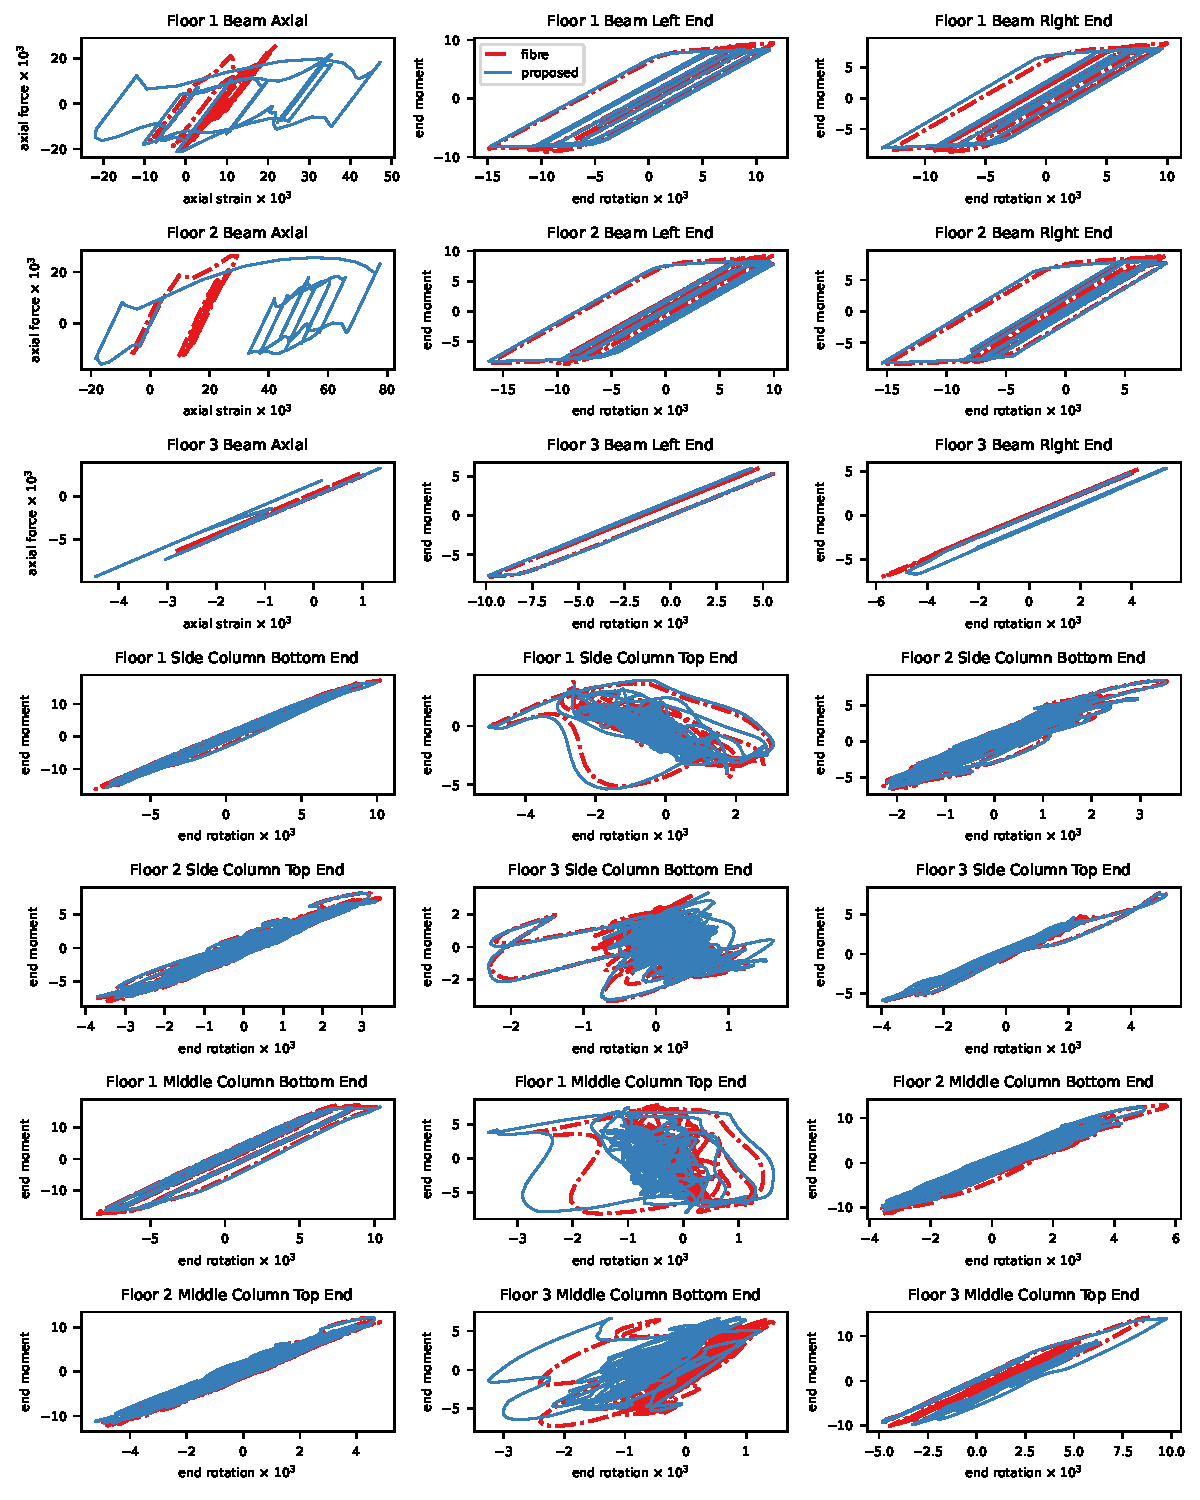
\includegraphics[width=.99\textwidth]{MODELS/FRAME/RESULT/FRAME.RESULT}
\caption{Hysteresis of frame members}\label{fig:hys}
\end{figure}
\begin{figure}[p]
\centering\footnotesize
\includegraphics[page=15]{PICCOLLECTION}
\caption{Different rules of kinematic hardening evolution of a 2D beam.}\label{fig:nm_component_kin}
\end{figure}
\end{document}